% Discussion

\glsresetall
\chapter{Discussion}

Analysis of the spectrograms show a mark that can be high in energy or be a trench in the signal. It is too early to assume this is the \gls{tune} but it is still very encouraging. It is possible to assess the feasibility of the tune measurement using \gls{GPU}.

\section{Observation}

During the three \glspl{MD} we acquired around 50 giga-bytes with both beams and both planes. This data was acquired in XML files and stored on the \gls{CERN} infrastructure. XML was chosen as it is easily accessible by both custom and commercial data analysis software.

Matlab was used as the first tool to check the data and try different algorithms but in the end the custom software was ready in time and found to be flexible enough. In the end Matlab was only used for checking and test purposes and all the analysis and discussion is based on the result obtained with the data analysis software (described in section~\ref{sec:data_analysis_software}).

\subsection{Without damper}

When the \gls{ADT} is off line there is a clear mark on the tune as shown in Figure~\ref{fig:adt_off}. There is still discussion as to whether it is the tune or just a ripple of the tune. Some tests could still be made, crosschecking with the \gls{BBQ}, changing the tune and looking in real time.

\begin{figure}[H]
\caption{Spectrogram with ADT off on the 16 October 2012 on vertical beam 1 before the ramp, 6 bunches 10 accumulations}
\label{fig:adt_off}
\centering
%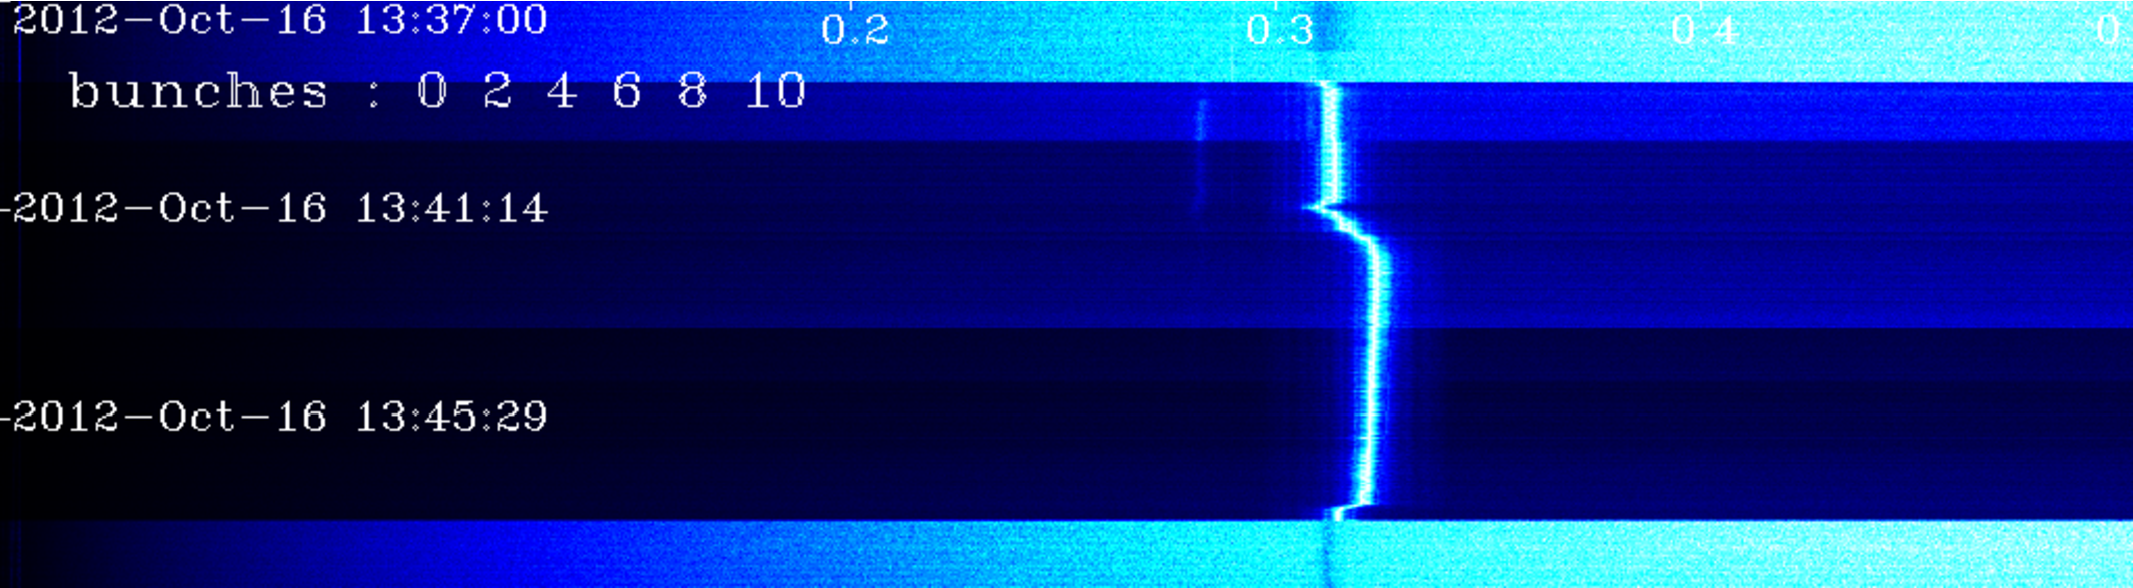
\includegraphics[scale=0.3]{md-121016-vb1-m1-6bunches-10acc-1337-1349-ADT-off.pdf}
\end{figure}

These observations are consistent with the gated-\gls{BBQ} result of 2012~\cite{Valuch12} and show that we can acquire the tune with the \gls{ADT} and get a clear bunch-by-bunch view of the tune even for only one bunch as shown in Figure~\ref{fig:bunch_0_adt_off}.

\begin{figure}[H]
\caption{Spectrogram with ADT off on the 16 October 2012 on horizontal beam 1 before the ramp, 1 bunch (0) 8 accumulations}
\label{fig:bunch_0_adt_off}
\centering
%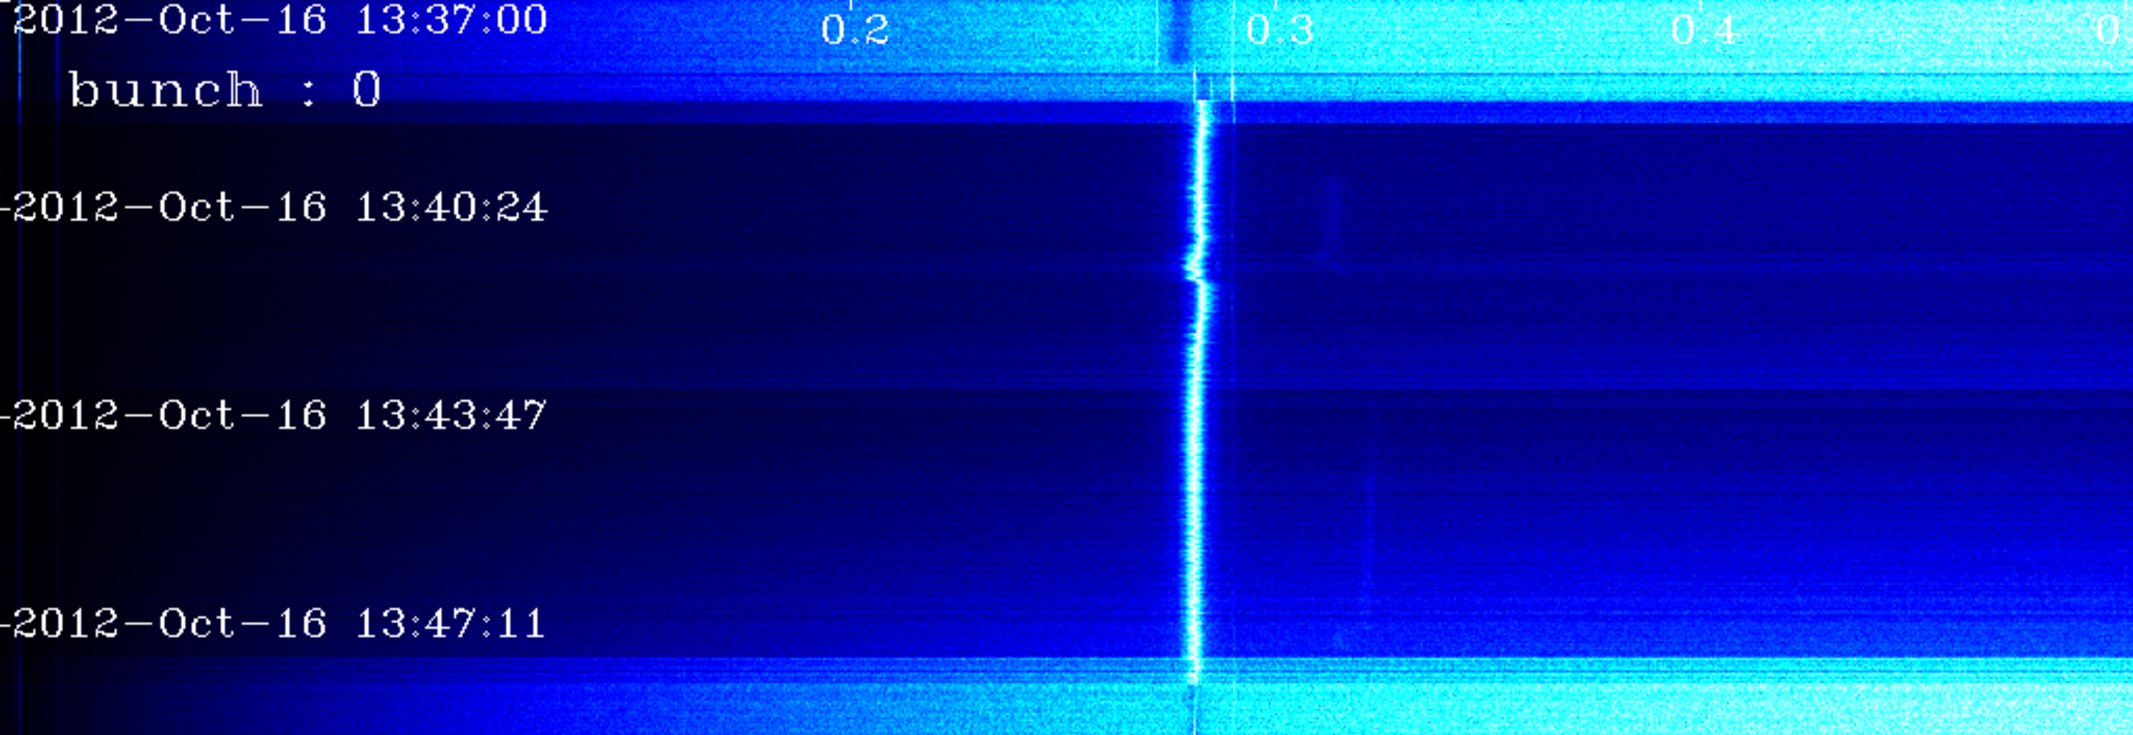
\includegraphics[scale=0.3]{md-121016-hb1-m1-bunch000001-8acc-1337-1349.pdf}
\end{figure}

\subsection{With damper}

When the \gls{ADT} is working the oscillations of the beam are damped by it, as a result the tune is less visible. But we should be able to see the effect of the tune on the damper if the damper is well adjusted to the beam. This mean that we should see a clear gap in the frequency around the tune frequency (or at the frequency at which the damper is operating, a frequency that should be close to the tune but not necessary be the tune itself).

This corresponds to the spectrogram we see during operation as shown in Figure~\ref{fig:ramp}. We also see in this figure the energy ramp before collision. Before putting the beam in collision we do a squeeze (operation during which we compress the beam size in the interaction points, where the experiments are). The squeeze is changing the tune and we can see it on the spectrogram around 14h03 on the figure~\ref{fig:ramp}.

\begin{figure}[H]
\caption{Spectrogram with damper, on the 16 October 2012 on vertical beam 1 during the ramp, 6 bunches 10 accumulations}
\centering
\label{fig:ramp}
%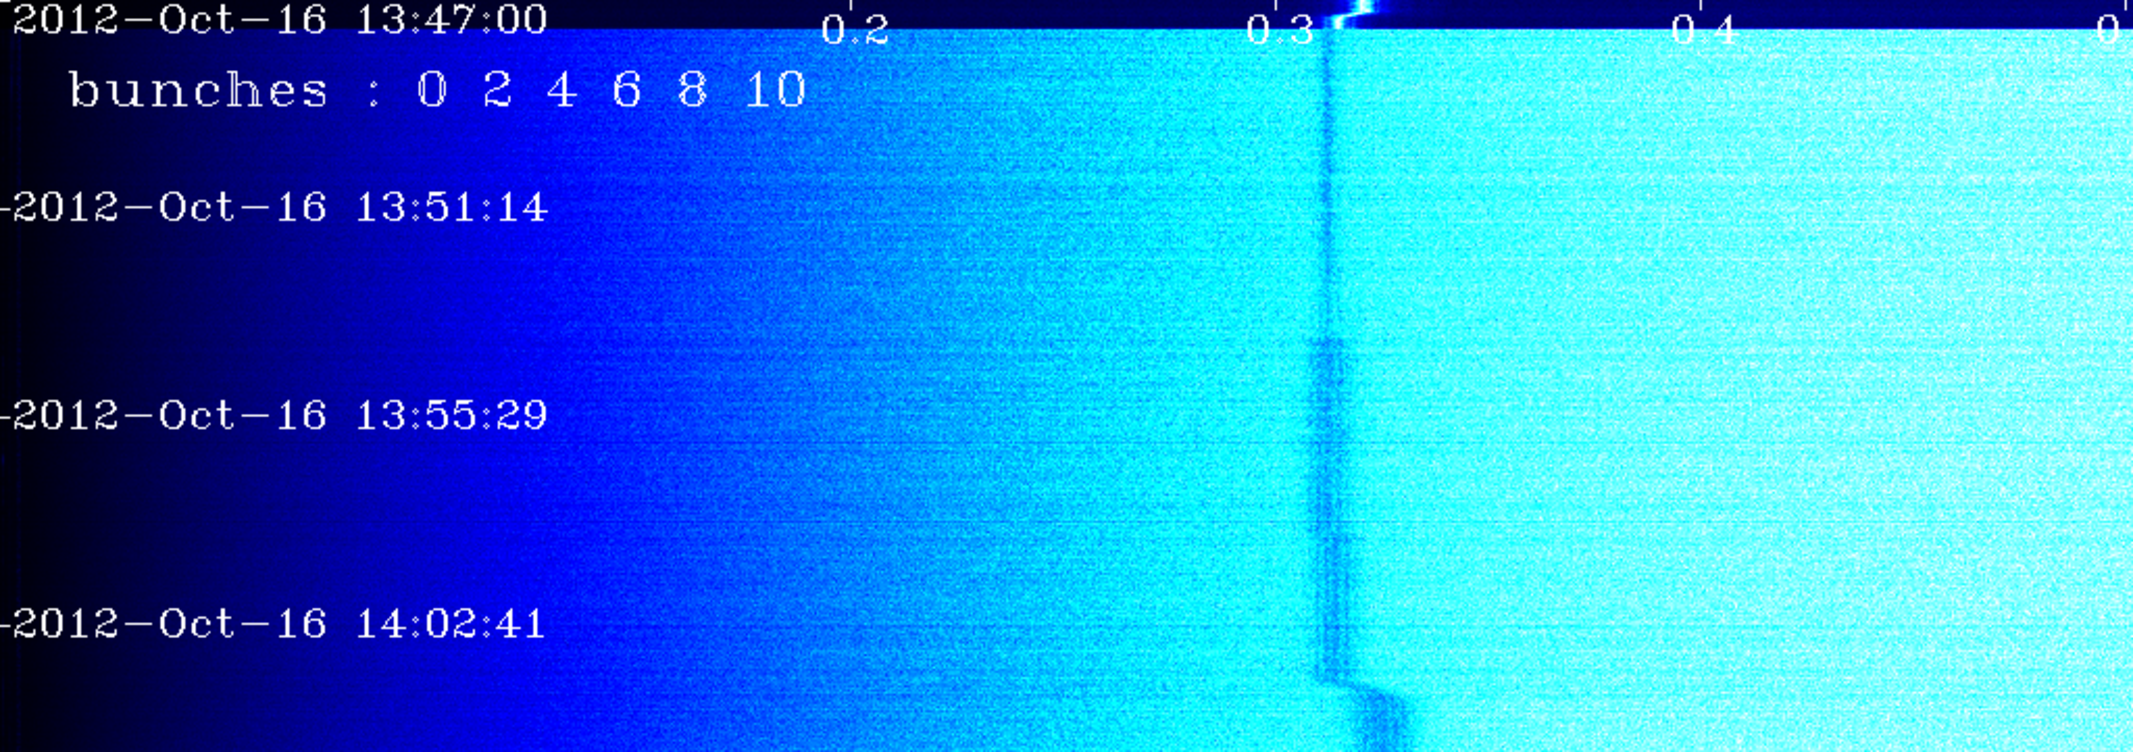
\includegraphics[scale=0.3]{md-121016-vb1-m1-6bunches-10acc-1347-1405-ramp.pdf}
\end{figure}

This could give us a good acquisition of the \gls{tune} during operation even when \gls{ADT} is on. This acquisition is made bunch-by-bunch. A question that is still open is how much is it sensitive to the way the \gls{ADT} is set up. This has still to be tested in the machine by moving the tune while the \gls{ADT} is in operation and see if the signal follows the tune.

\section{Data flow}

As the hardware is not present yet, the time and bandwidth of the whole system has to be estimated to see if it is feasible with the constraints we have as explained in the introduction. Estimation of the bandwidth and data flow is shown in Figure~\ref{fig:data_flow}.

\begin{figure}[H]
\caption{Acquisition data flow}
\label{fig:data_flow}
\centering
%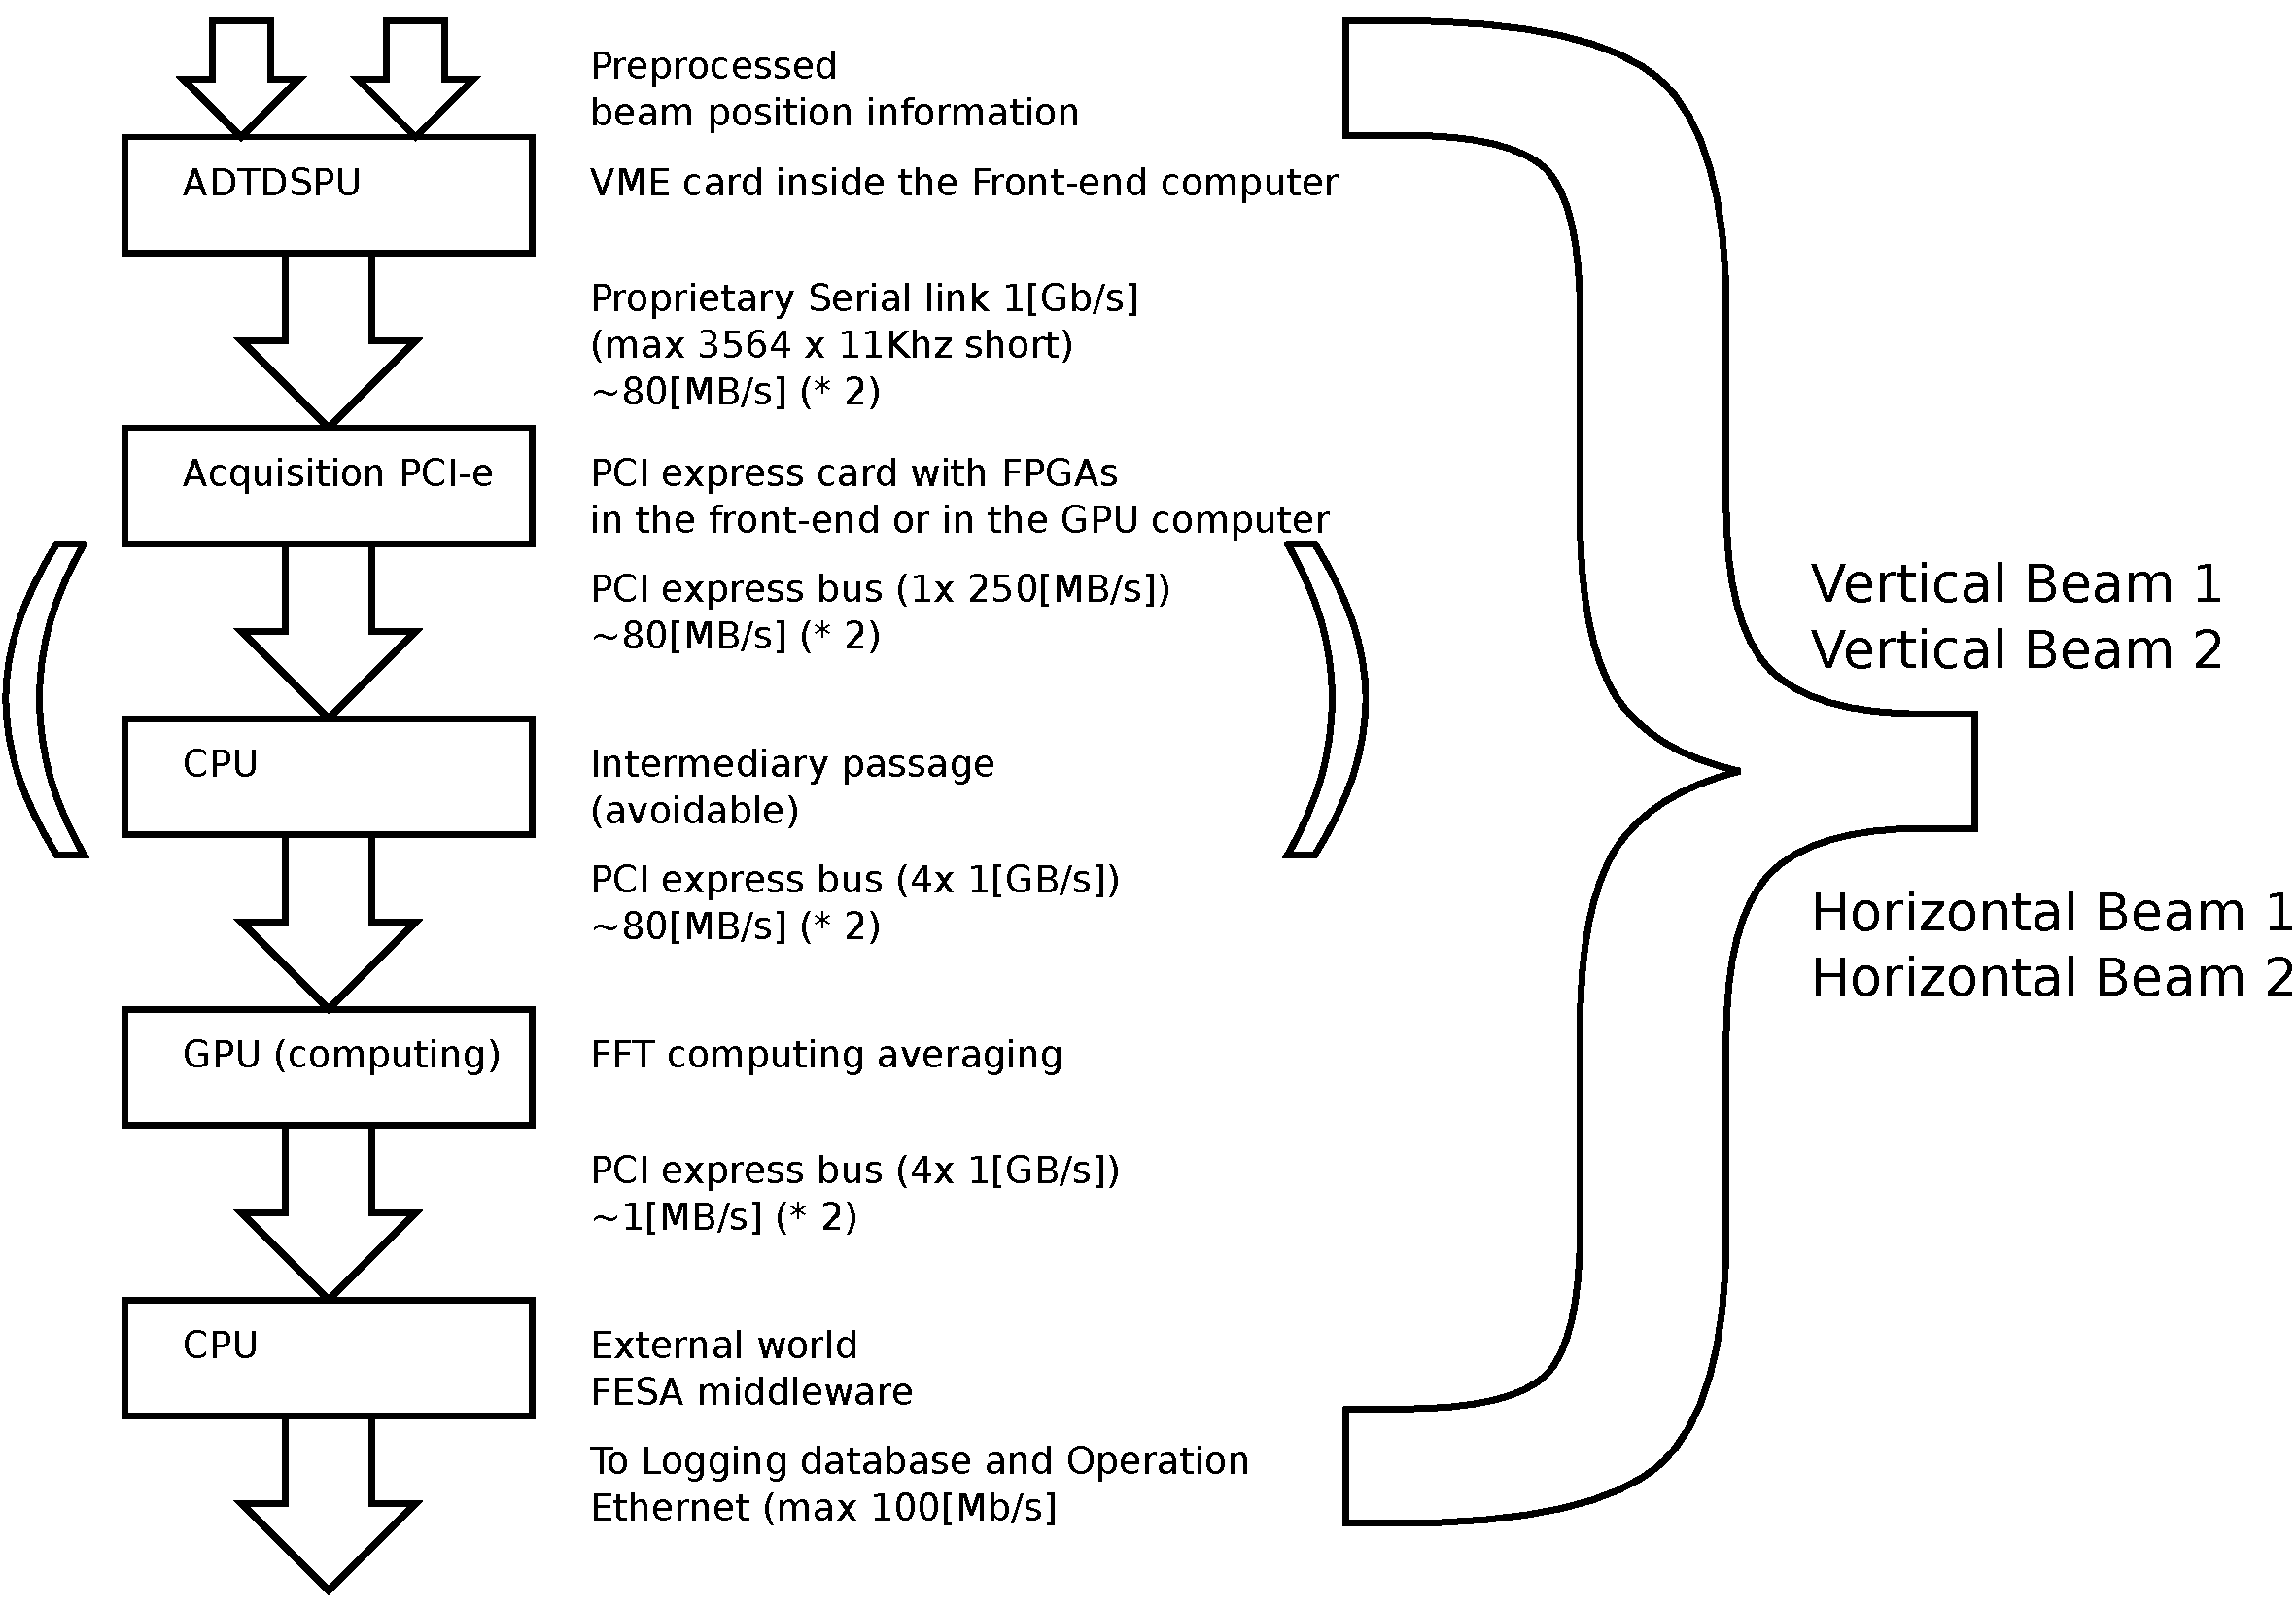
\includegraphics[scale=0.3]{dataflow.pdf}
\end{figure}

The data has to move from the acquisition card to the GPU by a series of steps, first from the card to the PCI crate (which contains the actual \glspl{GPU}). The problem being that the acquisition card is a \gls{VME} card and the VME bus is too slow to allow the full data to be streamed to the \gls{CPU}. 

We will use the giga-bit serial link already present on the VME
card. A receiver card will then receive the data in the PCI crate and
send it either directly to the \gls{GPU} memory or to the \gls{CPU}
and then to the \gls{GPU} memory.

The \gls{GPU} will make the computations necessary for the \gls{tune} measurement and will copy the results back to the \gls{CPU}.

As a final step we will use Ethernet to transmit the data back to the control room and eventually make the corrections needed.

\section{Hardware}

The present hardware does not allow us to acquire all the \glspl{bunch} of the machine and is in fact limited by constraints of the \gls{VME}. We have to upgrade various part of the hardware and to add the new computing device in order to be able to make on-line computation.

\subsection{ADT Acquisition boards}

The \gls{ADTDSPU} card will be redesigned and remade during the long shutdown 1 (\gls{LHC} upgrade from beginning of 2013 to 2015). It will be an upgrade of the whole card with \gls{tune} measurement and other necessary features in mind.

\subsection{Serial link interface}

A serial link receiver has to be chosen and put into place in the new computing device to be able to receive the data and pass them to the \gls{GPU}. This card has to be fast enough to get the serial data from the serial link that comes from the ADTDSPU, have a PCI-express interface and \gls{SFP} interface on the front panel. 

It should also have a fast FPGA to de-serialize the bunch positions and send them to the PCI-express bus. To be able to communicate with the CPU, Linux drivers (with sources) have to be present.

A market survey revealed that commercial cards can fulfill our needs.

\begin{figure}[H]
\caption{Nallatech PCIe-180}
\label{fig:nallatech}
\centering
%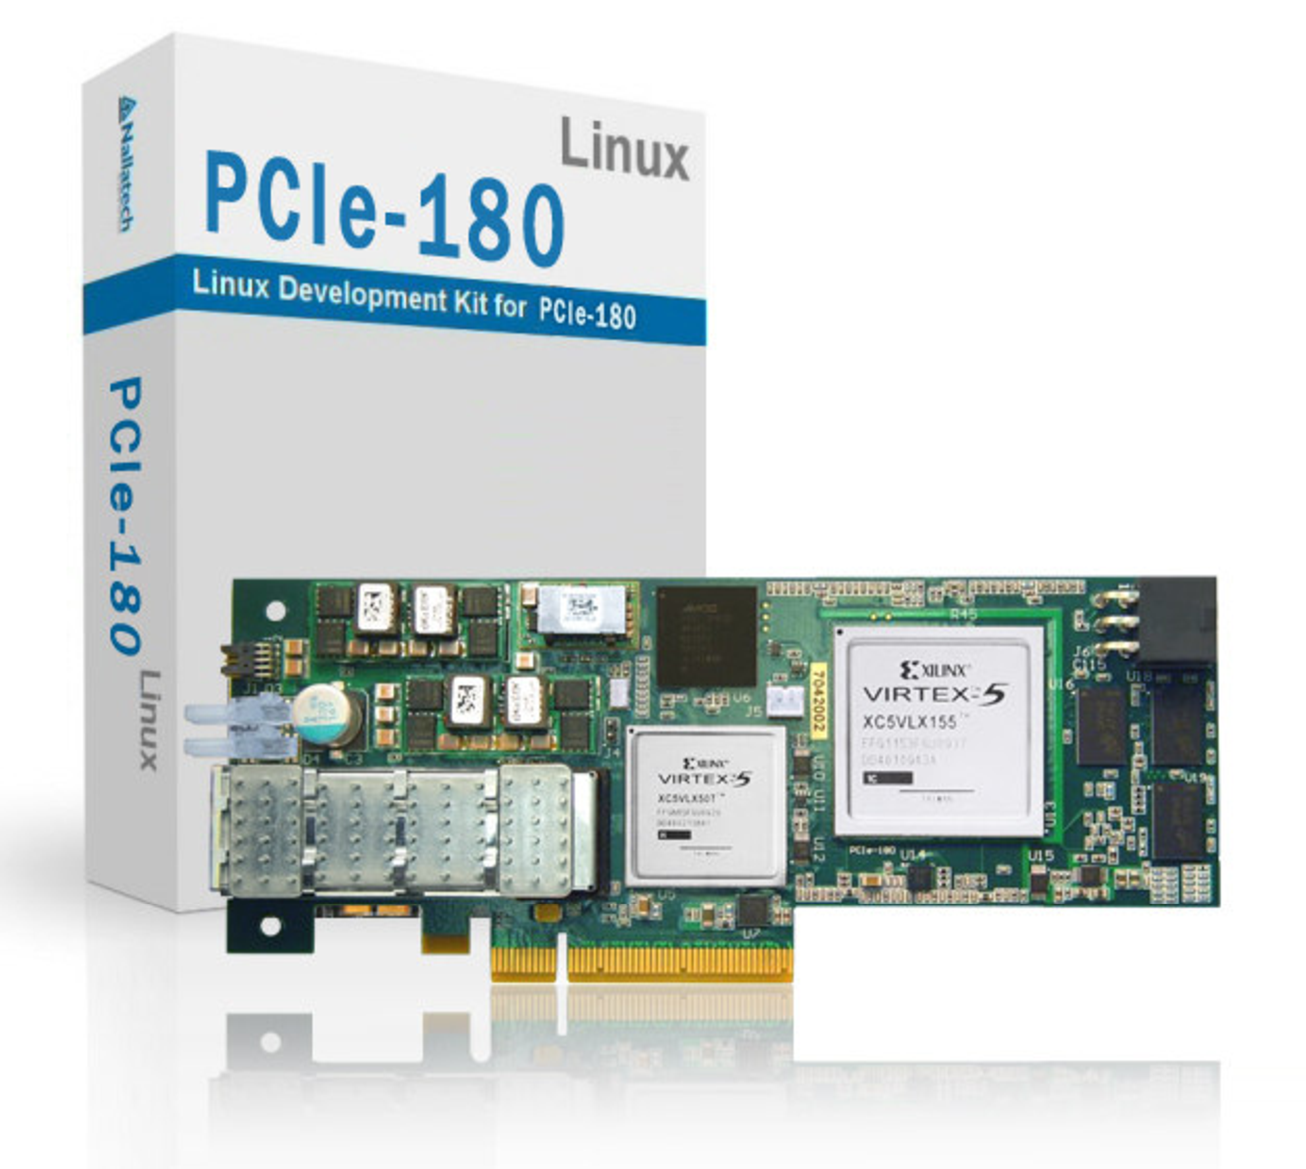
\includegraphics[scale=0.3]{Nallatech_PCIe-180.pdf}
\end{figure}

\gls{CERN} proposes a card that is made by \gls{CO} which could make a good match.

\begin{figure}[H]
\caption{CERN Simple FMC carrier (SPEC)}
\label{fig:spec}
\centering
%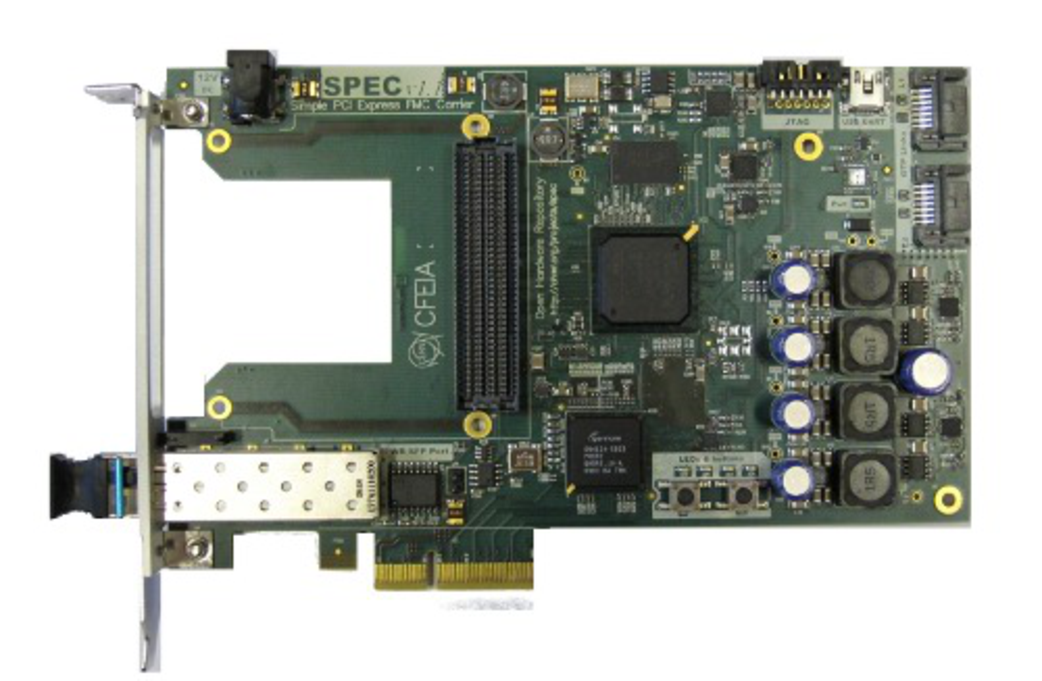
\includegraphics[scale=0.3]{spec_top.pdf}
\end{figure}

Table~\ref{tab:receiver_cards} show the different commercial and CERN solutions.

\begin{table}[H]
\caption{PCIe Giga bit link serial receiver card candidates}
\label{tab:receiver_cards}
\centering
\begin{tabular}{|ll|c|l|c|}
\hline
Name & Manufacturer & SFP & FPGA & Drivers \\
\hline
\hline
SPEC & CERN & 1 & Spartan-6 & yes \\
\hline
Virtex-5 LXT ML555 & Xilinx & 2 & Spartan-5 & no \\
\hline
Xilinx Virtex 6 & Hitech Global & 2 & Spartan-6 & no \\
\hline		
PCIe-287N & Nallatech & 4 & Kintex-7 * 2 & yes \\		
PCIe-180 & Nallatech & 2 & Virtex-5 & yes \\
\hline
\end{tabular}
\end{table}

For the moment the ``Nallatech PCIe-180'' seams to be the best match and we will probably order one to start testing with the present test setup.

\subsection{GPUs}

We need a computing device with at least 2 PCIe slots, one for the serial link receiver and one for the \gls{GPU} card. It should be a standardized crate with a powerful \gls{CPU} and possible expansion. Space has to be found in SR4, for either a full crate or a smaller one.

We will probably start with a standard graphics card and then upgrade to a professional computing \gls{GPU} card (like NVIDIA Tesla series~\cite{nvidia}).

\section{Software}

Some software upgrade and redeployment is still necessary before the operational version is fully commissioned. New hardware will need new drivers and the software will have to be changed accordingly.

\subsection{Drivers}

The drivers for the \gls{ADT} acquisition card will need some updating, changing the memory map and adjusting the drivers for the control registers. This should be quite straightforward.

A driver for the Serial link receiver card will be needed. If we use one that is made inside \gls{CERN} we can have it made by the controls group (CO). In case we buy an off the shelf solution we will have to make the driver in-house using the driver framework and the tools we have.

\subsection{OpenCL}

The present \gls{OpenCL} code is able to compute the \gls{FFT} but we could try other algorithms in the future including hardware accelerated \gls{SVD}. This would require some new \gls{OpenCL} development.

\subsection{Front-end}

It will be necessary to develop new software to control the new hardware. The \gls{ADTDSPU} board is going to be changed and we are going to build a new computing front-end with a custom serial link receiver and a \gls{GPU}. New drivers and software to stream data from the receiver card to the \gls{GPU} will be needed.

\section{Intermediate and Final setup}

A normal computer with a decent \gls{CPU} can be estimated to cost around 2'000 SFR and a high-end \gls{GPU} is around 1'000 SFR. The receiver card should have a similar cost.

In case we have to move to rackable \gls{CPU} and a professional \gls{GPU} the price can go up to around 10'000 SFR per crate. This is still much cheaper than a \gls{VME} crate and custom cards.

\subsection{First prototype}

First prototype could be a standard computer with the receiver card and a graphics card \gls{GPU}. The idea is to test the hardware, and decide on the final setup.

This test will be made on the \gls{ADT} test setup in the laboratory and will be fed from the new version of the \gls{ADTDSPU} card.

\subsection{Final version}

At the \gls{LHC} restart in 2015, four crates will be deployed in \gls{SR4}, one for each ring and for each plane.

It will probably be built using industrial crates with a certain number of \glspl{GPU} and a serial link receiver card. 

If space allows, the test crate may be moved as well to be used on the test acquisition crate in \gls{SR4}.
